\documentclass[10pt,twocolumn,letterpaper]{article}

\usepackage{cvpr}
\usepackage{times}
\usepackage{epsfig}
\usepackage{graphicx}
\usepackage{amsmath}
\usepackage{amssymb}
\usepackage{subfiles}
\usepackage{color}
\usepackage{enumitem}
\usepackage{dsfont}
\usepackage{booktabs}
\usepackage{float}
\usepackage{capt-of,etoolbox}
\usepackage{graphicx}
\usepackage{caption}
\usepackage{subcaption}
\usepackage{multirow}
\usepackage{arydshln}

\definecolor{MyDarkBlue}{rgb}{0.08,0.02,0.5}
\definecolor{MyLightBlue}{rgb}{0,0.08,0.8}
\definecolor{MyDarkGreen}{rgb}{0.02,0.50,0.02}
\definecolor{MyDarkRed}{rgb}{0.7,0.02,0.02}
\definecolor{MyDarkOrange}{rgb}{0.40,0.2,0.02}
\definecolor{MyDarkMagenta}{rgb}{0.337,0,0.827}
\definecolor{MyDarkGray}{rgb}{0.5,0.5,0.5}
\newcommand{\gray}[1]{\textcolor{MyDarkGray}{#1}}
\newcommand{\tbfit}[1]{\textbf{\textit{#1}}}
\newcommand{\tbfu}[1]{\textbf{\underline{#1}}}

%\setlength{\textfloatsep}{1.3em}
%\setlength{\floatsep}{0em}

\renewcommand{\paragraph}[1]{\vspace{5px} \noindent \textbf{#1} \ \ }
% Include other packages here, before hyperref.

% If you comment hyperref and then uncomment it, you should delete
% egpaper.aux before re-running latex.  (Or just hit 'q' on the first latex
% run, let it finish, and you should be clear).
\usepackage[pagebackref=true,breaklinks=true,letterpaper=true,colorlinks,bookmarks=false,draft]{hyperref}

\cvprfinalcopy % *** Uncomment this line for the final submission

\def\cvprPaperID{299} % *** Enter the CVPR Paper ID here
\def\httilde{\mbox{\tt\raisebox{-.5ex}{\symbol{126}}}}

% Pages are numbered in submission mode, and unnumbered in camera-ready
% \ifcvprfinal\pagestyle{empty}\fi
\setcounter{page}{1}
\begin{document}


%%%%%%%%% TITLE
% \title{Learning a Perceptual Distance Metric}
\title{The Unreasonable Effectiveness of Deep Features as a Perceptual Metric}

\author{Richard Zhang$^{1}$ \hspace{3mm} Phillip Isola$^{12}$ \hspace{3mm} Alexei A. Efros$^{1}$\\
$^{1}$UC Berkeley \hspace{3mm} $^{2}$OpenAI\\
{\tt\small \{rich.zhang, isola, efros\}@eecs.berkeley.edu}
\and
Eli Shechtman$^{3}$ \hspace{3mm} Oliver Wang$^{3}$\\
$^{3}$Adobe Research\\
{\tt\small \{elishe,owang\}@adobe.com}
}

\twocolumn[{%
\vspace{-45px}
\renewcommand\twocolumn[1][]{#1}%
\maketitle
\centering
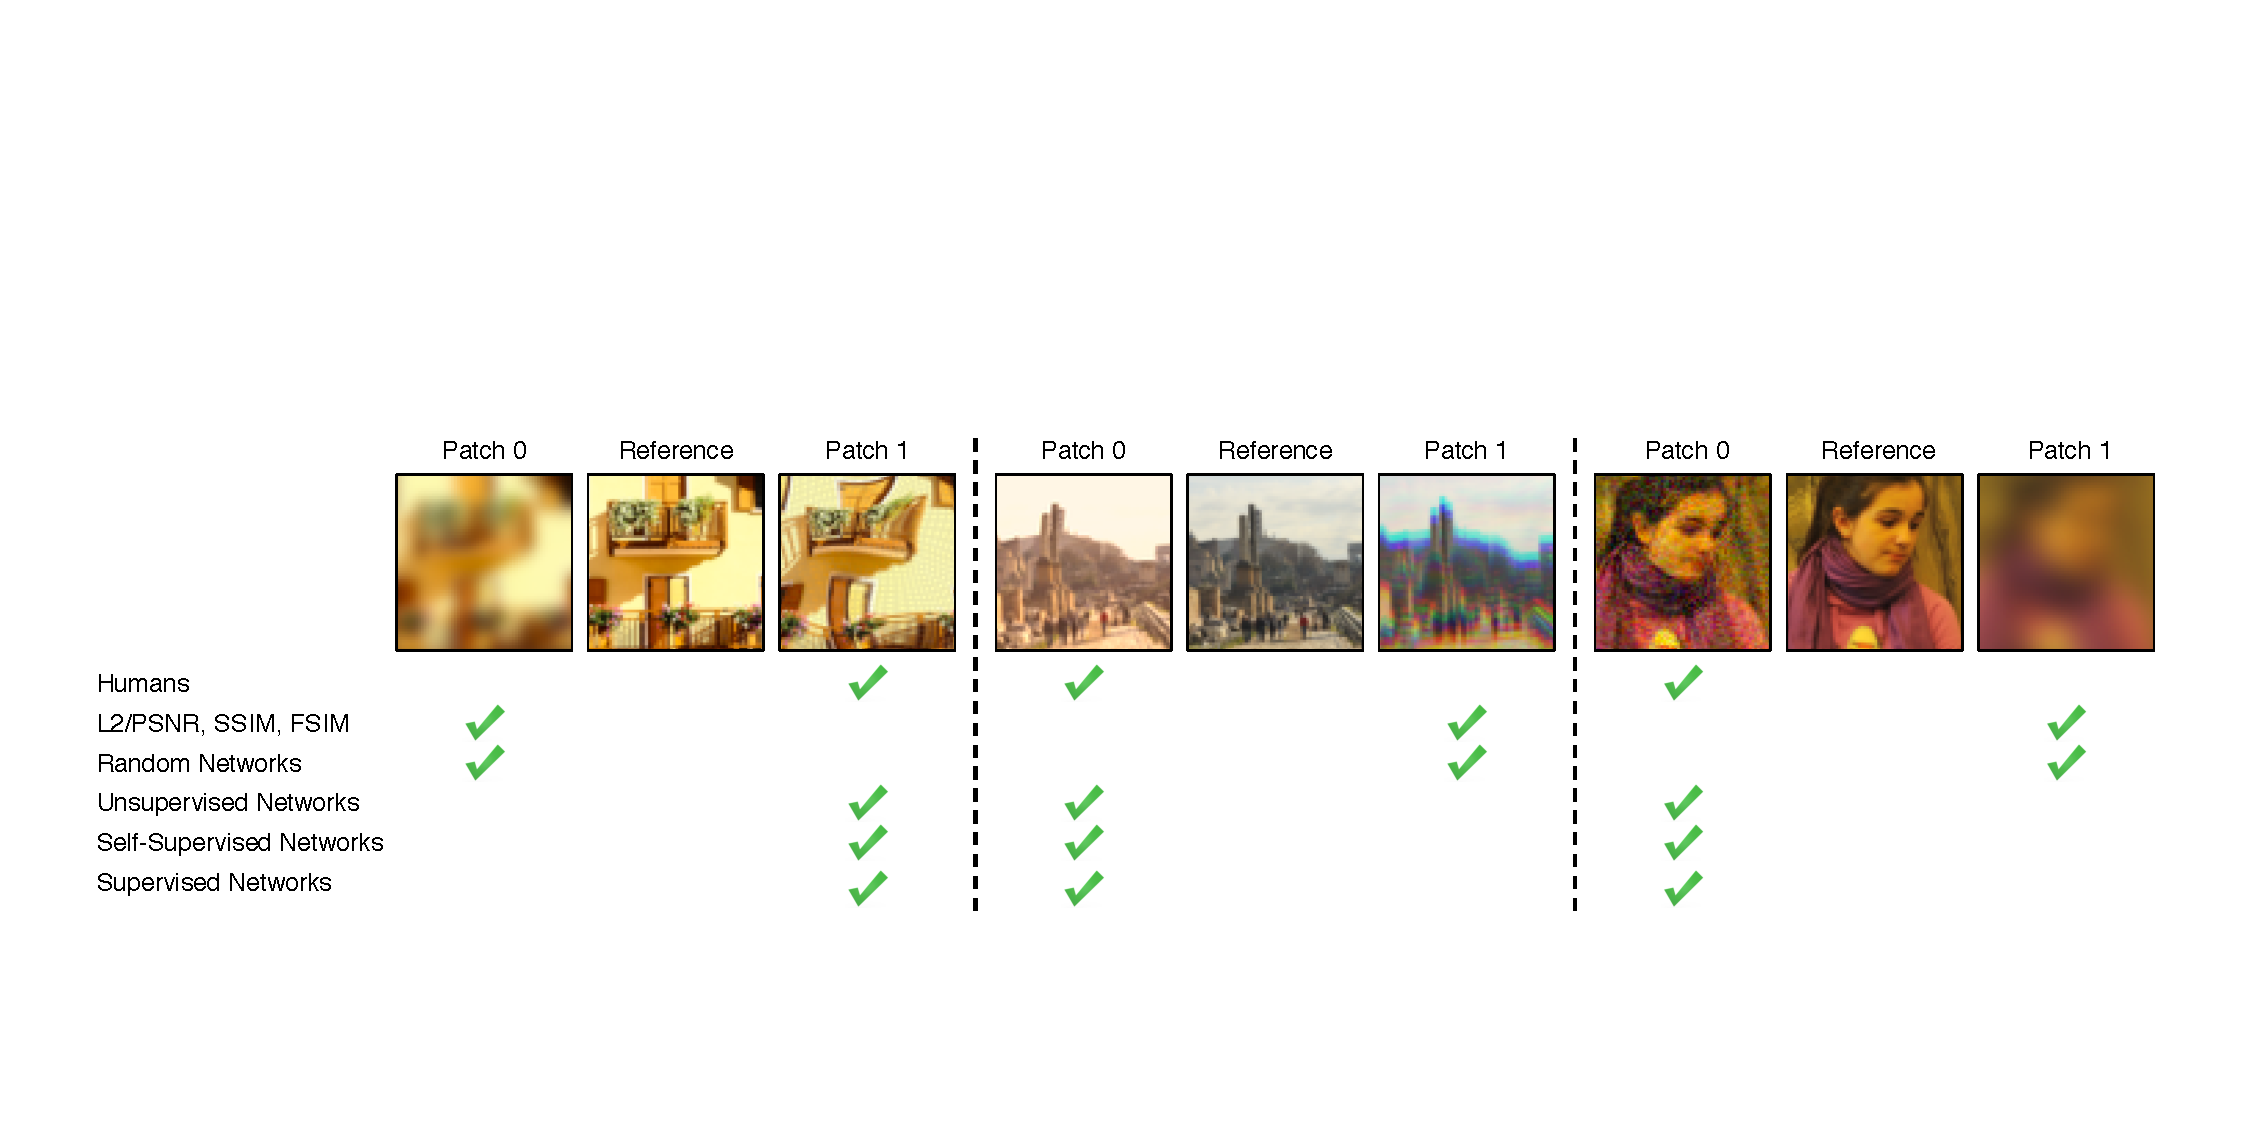
\includegraphics[width=1.\linewidth]{imgs/fig1_v2.pdf}
\vspace{-16px}
\captionof{figure}{\label{fig:fig1}
\textbf{Which patch (left or right) is ``closer" to the middle patch in these examples?} In each case, the traditional metrics (L2/PSNR, SSIM, FSIM) disagree with human judgments. 
But deep networks, even across architectures (Squeezenet~\cite{iandola2016squeezenet}, AlexNet~\cite{krizhevsky2014one}, VGG~\cite{simonyan2014very}) and supervision type (supervised~\cite{russakovsky2015imagenet}, self-supervised~\cite{donahue2016adversarial, noroozi2016unsupervised,pathak2017learning,zhang2017split}, and even unsupervised~\cite{krahenbuhl2015data}), provide an \textit{emergent embedding} which agrees surprisingly well with humans. We further calibrate existing deep embeddings on a large-scale database of perceptual judgments; models and data can be found at \url{https://www.github.com/richzhang/PerceptualSimilarity}.}
\vspace{10px}
}]

%\maketitle
%\thispagestyle{empty}

%%%%%%%%% ABSTRACT

\subfile{sections/0_abstract}

%%%%%%%%% BODY TEXT
\subfile{sections/1_introduction}

\subfile{sections/2_methods}

\subfile{sections/3_experiments}

\subfile{sections/4_conclusions}

\vspace{-1mm}
{\paragraph{Acknowledgements} This research was supported, in part, by grants from Berkeley Deep Drive, NSF IIS-1633310, and hardware donations by NVIDIA. We thank members of the Berkeley AI Research Lab and Adobe Research for helpful discussions. We thank Alan Bovik for his insightful comments. We also thank Radu Timofte, Zhaowen Wang, Michael Waechter, Simon Niklaus, and Sergio Guadarrama for help preparing data. RZ is partially supported by an Adobe Research Fellowship and much of this work was done while RZ was an intern at Adobe Research.}

{\small
\bibliographystyle{ieee}
\bibliography{egbib}
}

\appendix
\subfile{sections/A_supplemental}
\subfile{sections/B_model}
\subfile{sections/C_tid}
\subfile{sections/D_changelog}

\end{document}
